\documentclass[aps, prc, reprint, amsmath, groupedaddress, nofootinbib]{revtex4-1}

\usepackage[utf8]{inputenc}
\usepackage{hyperref}
\usepackage{amsmath}
\usepackage{amssymb}
\usepackage{amsfonts}
\usepackage{tabularx}
\usepackage{booktabs}
\usepackage{graphicx}
\usepackage{color}
\usepackage{multirow}
\usepackage[inline]{enumitem}
\graphicspath{{fig/}}
\definecolor{theblue}{RGB}{0,50,230}
\usepackage{appendix}
\hypersetup{
  colorlinks=true,
  linkcolor=theblue,
  citecolor=theblue,
  urlcolor=theblue
}


\newcommand{\trento}{T\raisebox{-0.5ex}{R}ENTo}
\newcommand{\nch}{N_\text{ch}}
\newcommand{\sqrts}{\sqrt{s_{NN}}}
\newcommand{\T}{\tilde{T}}
\newcommand{\paddedhline}{\noalign{\smallskip}\hline\noalign{\smallskip}}
\newcommand{\dnchdy}{dN_\text{ch}/d\eta}
\newcommand{\dndypP}{dN_\text{pPb}/d\eta}
\newcommand{\dndyPP}{dN_\text{PbPb}/d\eta}
\newcommand{\x}{\mathbf x}
\newcommand{\y}{\mathbf y}
\newcommand{\z}{\mathbf z}
\newcommand{\trans}{^\intercal}

\newcommand{\Raa}{R_{AA}}
\newcommand{\vv}{v_2\{2\}}
\newcommand{\vvv}{v_3\{2\}}
\newcommand{\vnv}{v_n\{2\}}
\newcommand{\ppi}{\frac{\partial}{\partial p_i}}
\newcommand{\ppj}{\frac{\partial}{\partial p_j}}
\newcommand{\ppl}{\frac{\partial}{\partial p_l}}
\newcommand{\Kpara}{\kappa_{\|}}
\newcommand{\Kperp}{\kappa_{\perp}}
\newcommand{\Ppara}{\hat{P}^{\|}}
\newcommand{\Pperp}{\hat{P}^{\perp}}

\begin{abstract}
Open heavy-flavor production in relativistic heavy-ion collisions provides valuable information about the quark-gluon plasma (QGP).
Current observation of open charm in heavy-ion collisions shows unexpectedly large momentum anisotropy and small nuclear modification factor, posing a challenge to the theoretical understanding of the nature of coupling between heavy quark and the medium.
Linear Boltzmann transport and Langevin diffusion are two popular kinetic models for heavy quark in-medium propagation.
In this work, we develop a hybrid heavy quark transport model that combines the strengths of each approach: 
heavy quarks are evolved with Langevin diffusion using an empirical diffusion constant, while rare but important scattering processes are described using linear Boltzmann equations with perturbative matrix elements.
In such a setup, the Langevin component can be understood as a complementary contribution to the linear Boltzmann equation in cases where perturbative calculation may be inadequate to describe all the interactions.
Both elastic and inelastic scatterings are included in the Boltzmann component.
The Landau-Pomeranchuk-Migdal effect is treated effectively via gluon formation time and detailed balance is imposed between gluon emission and absorption.
Finally, the QGP evolution is obtained by a 2+1D relativisic viscous hydrodynamic calculation.
With the hybrid model, we study the heavy flavor momentum anisotropic, nuclear modification factor, and correlation observables in A-A collisions at the RHIC and the LHC energies.
Comparing to available D and B meson data, we constrain the diffusion constant of the Langevin component.

\end{abstract}


\begin{document}


\title{A hybrid heavy quark transport model in a quark-gluon plasma that couples linear Boltzmann equation and Langevin diffusion dynamics}
\author{Weiyao Ke}
\author{Yingru Xu}
\author{Steffen A.\ Bass}
\affiliation{Department of Physics, Duke University, Durham, NC 27708-0305}
\date{\today}
\maketitle

\section{Introduction}

\section{Heavy quark propagation in a QGP}

\subsection{The linear Boltzmann equation and scatterings}
Heavy quark's large mass ($M \gg T$) makes it a good quasi-particle with a dilute distribution $e^{-\beta M} \ll 1$ compared to other components of the QGP.
Neglecting the back reaction from heavy quark to the medium, the full Boltzmann equations can be linearized for heavy quark propagation.
\begin{eqnarray}
  \frac{\partial}{\partial t}f_Q - \frac{\vec{p_1}}{E_1}\cdot\nabla f_Q  = C_i^{2\rightleftharpoons 2}[f_Q] + C_i^{2\rightleftharpoons 3}[f_Q]
\end{eqnarray}
On the right, we include elastic and inelastic collision terms, involving heavy quark, light quark and gluon distribution functions and the scattering matrix elements.
To solve the equation with an ensemble of test particles, each particles reacts with medium particles with collisions rates,
\begin{eqnarray}
    R_{i=q,\bar{q},g}^{1+2 \rightarrow 3+4} &=& \frac{d_i}{2E_1\nu_i !} \int d \Gamma_2 d \Gamma_3 d \Gamma_4 f_i(p_2) 
   \nonumber
  \\&& {(2\pi)}^4\delta^{(4)}(p_{\textrm{in}} - p_{\textrm{out}})  \overline{|M_{Q+i \rightleftharpoons Q+i}|^2},
   \nonumber
  \\
  R_{i=q,\bar{q},g}^{1+2 \rightarrow 3+4+k} &=& \frac{d_i}{2E_1\nu_i !} \int d \Gamma_2 d \Gamma_3 d \Gamma_4 d \Gamma_k f_i(p_2) 
   \nonumber
  \\&& {(2\pi)}^4\delta^{(4)}(p_{\textrm{in}} - p_{\textrm{out}})\overline{|M_{Q+i \rightleftharpoons Q+i+g}|^2},
  	 \nonumber
  \\
  R_{i=q,\bar{q},g}^{1+2+k \rightarrow 3+4} &=& \frac{d_i d_g}{2E_1\nu_i !} \int d \Gamma_2 d \Gamma_3 d \Gamma_4 d \Gamma_k f_i(p_2)f_g(k)
   \nonumber
  \\&& {(2\pi)}^4\delta^{(4)}(p_{\textrm{in}} - p_{\textrm{out}})\overline{|M_{Q+i \rightleftharpoons Q+i+g}|^2}.
  	 \nonumber
\end{eqnarray}
$d\Gamma = dp^3/2E/(2\pi)^3$ is the invariant phase space integration, $d_i$ counts the degeneracy of the incoming medium particle and $\nu_i$ counts the number of identical particles in the initial / final state of the collision.
The medium particle distribution functions are assumed to be classical and thermal, 
\begin{eqnarray}
f(p,x) = \exp\left(-\frac{p \cdot u(x)}{T(x)}\right).
\end{eqnarray}
The space-time profile temperature and velocity of the medium are obtained from the 2+1D viscous relativistic hydrodynamic calculations.

The first collision rate is called "elastic" in the sense that it conserves particle number.
Simiarly, the second and the third collision rates are "inelastic" as they do not conserve particle number, where heavy quark collide with meidum particle and at the same time radiates / absorbs a gluon.
The matrix-elements for these processes are calculated at leading order pQCD (see \ref{appendix:matrix-element}), with a leading order Debye mass screening the gluon and quark propagator to remove the infrared divergence,
\begin{eqnarray}
m_D^2 = \frac{4\pi\alpha_s}{3}(Nc+\frac{N_f}{2})T^2
\end{eqnarray}
The Debye mass $\sim gT$ can also be treated as a soft cut-off so that the screened matrix-elements only handle momentum transfer $\gtrsim gT$.
We used the leading order running coupling constant with three flavors of quark [cite BAMPS, etc] for the matrix-element,
\begin{eqnarray}
\alpha_s(\mu) = \frac{4\pi}{9}
\begin{cases}
\frac{1}{\ln\left(-\mu^2/\Lambda^2\right)},\hfill \mu^2 < 0 \\ 
\frac{1}{2} - \frac{1}{\pi}\arctan\left[\frac{\ln\left(\mu^2/\Lambda^2\right)}{\pi}\right],\mu^2 > 0
\end{cases}
\end{eqnarray}
The QCD scale is chosen to be $\Lambda = 200$~MeV.
In vacuum, the scale $\mu^2$ should be chosen as the typical momentum transfer $Q^2$ of that process.
However, for scatterings inside a medium characterized by temperature $T$, the typical scale should be cut-off by $T$ and we choose $\mu = \max\{Q, \nu\pi T \}$, with $\nu$ the only parameter we tuned in the linear Boltzmann transport component.

The inelastic processes that involve gluon radiation / absorption needs extra care. 
A gluon radiating off a heavy quark takes a finite formation time $\tau_f$ to be fully resolved from the source quark. During this time, the effect from multiple soft collisions contribute coherently at leading order.
Therefore, a proper treatment of the coherence needs careful re-summation of multiple soft collisions.
The destructive interference of multiple collisions leads to a suppression to the rate of gluon emission, known a the Landau-Pomeranchuk-Migdal (LPM) effect.
However, coherence effect is hard to implement in a Boltzmann equation transport model, where scatterings are treated as independent and local.
We adopt the way used in [Shanshan's paper] to effectively taking this into account via the formation time of the gluon,
\begin{eqnarray}
\tau_f = \frac{2x(1-x)E}{k_\perp^2 + x^2M^2 + (1-x)m_g^2}
\end{eqnarray}
where $m_g = m_D/\sqrt{2}$ is the gluon thermal mass.
This effective treatment of LPM effect restricts the phase space of the radiated/absorbed gluon in the calculation of scattering rates at time $t$,
\begin{eqnarray}
R(t) = \int (\cdots)d\Gamma_k \rightarrow \int (\cdots) 2\sin^2\left(\frac{t-t_0}{\tau_f}\right)d\Gamma_k,
\end{eqnarray}
where $t_0$ is the time of last radiation / absorption of gluon.
In this approach, a gluon radiation immediately after the last emission vertex is suppressed by the interference factor, and the differential scattering rate for gluon with momentum $k$ will not recover the incoherent limit until $t-t_i$ is comparable to $\tau_f$.
This procedure is of course not perfect, but captures the main impact of a finite formation time, for example the non-linear path-length dependence of energy loss.
Another consequences is that the inelastic collision term on the right-hand-side of the Boltzmann equation now depends on the history of evolution.
There is no guarantee that this modification does not alter the equilibrium solution.
However, we checked and confirmed that that as long as absorption processes are included, the true thermal equilibrium can be reached with acceptable precision.

\subsection{The diffusion dynamics}
The diffusion equation dynamics is solved by the Langevin equations.
In the post-point discretization scheme, these are,
\begin{eqnarray}
\Delta \vec{x}_i &=& \frac{\vec{p}_i}{E} \Delta t	\\
\Delta \vec{p}_i &=& -\Gamma \vec{p}_i \Delta t + \sqrt{\tensor{B}(p+\Delta p) \Delta t  }\vec{\xi}
\end{eqnarray}
$\Gamma$ is the Langevin drag term, and $\tensor{B}$ is the random force correlation matrix,
\begin{eqnarray}
B_{ij} = \Kpara \frac{p_i p_j}{p^2} + \Kperp \left(\delta_{ij} - \frac{p_i p_j}{p^2}\right)
\end{eqnarray}
To guarantee an ensemble of particles reaches the thermal equilibrium at $t\rightarrow \infty$, $\Gamma$ and $\kappa$ have to satisfy the Einstein relation in the post-point scheme,
\begin{eqnarray}
\Gamma &=& A + \frac{\partial \Kpara}{p^2} + \frac{2\sqrt{\Kpara\Kperp} - 2\Kperp}{p^2} \\
 &=& \frac{\Kpara}{2TE} - \frac{1}{p^2}\left( \sqrt{\Kpara} - \sqrt{\Kperp} \right)^2.
\end{eqnarray}

\subsection{A hybrid model}

\section{Benchmark calculation}
\begin{figure}
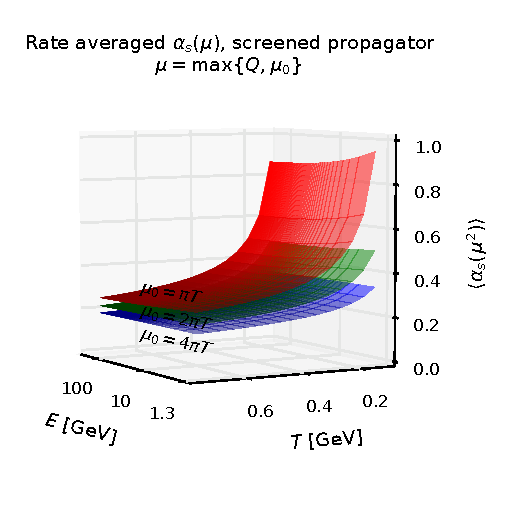
\includegraphics[width=\columnwidth]{charm-plot/avg_alphas.pdf}\\
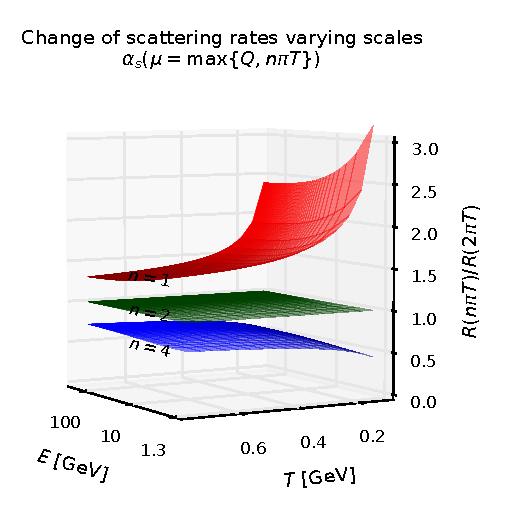
\includegraphics[width=\columnwidth]{charm-plot/Rscale.pdf}
\end{figure}

\begin{figure}
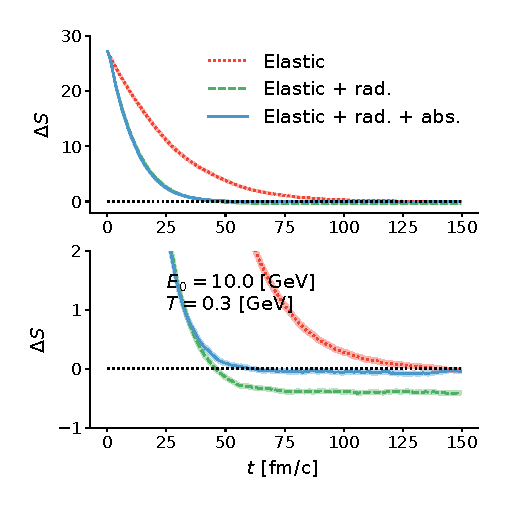
\includegraphics[width=\columnwidth]{charm-plot/thermalization.pdf}
\end{figure}

\begin{figure*}
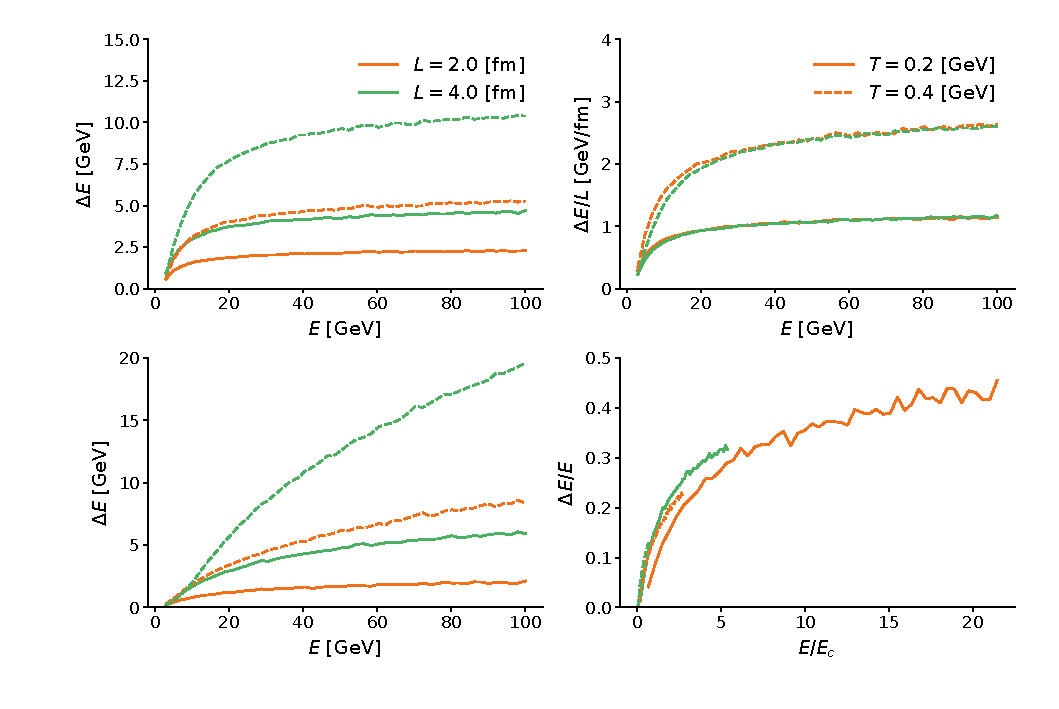
\includegraphics[width=\textwidth]{E_Eloss.pdf}\\
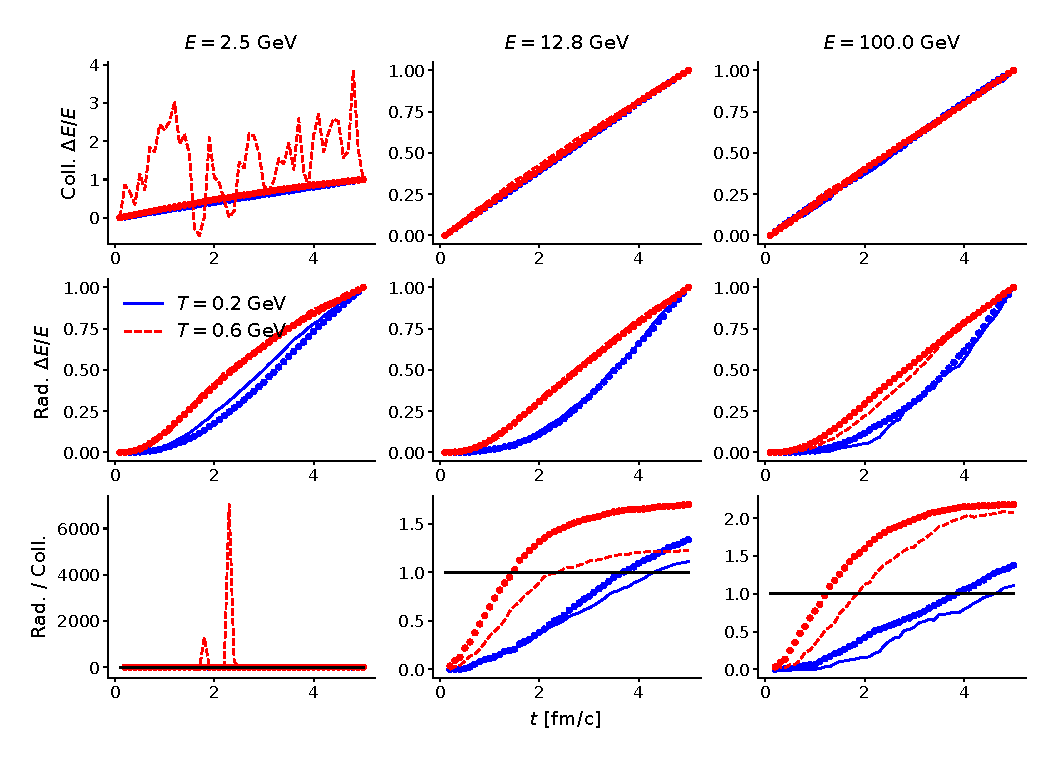
\includegraphics[width=\textwidth]{L_Eloss.pdf}
\end{figure*}

\begin{figure*}
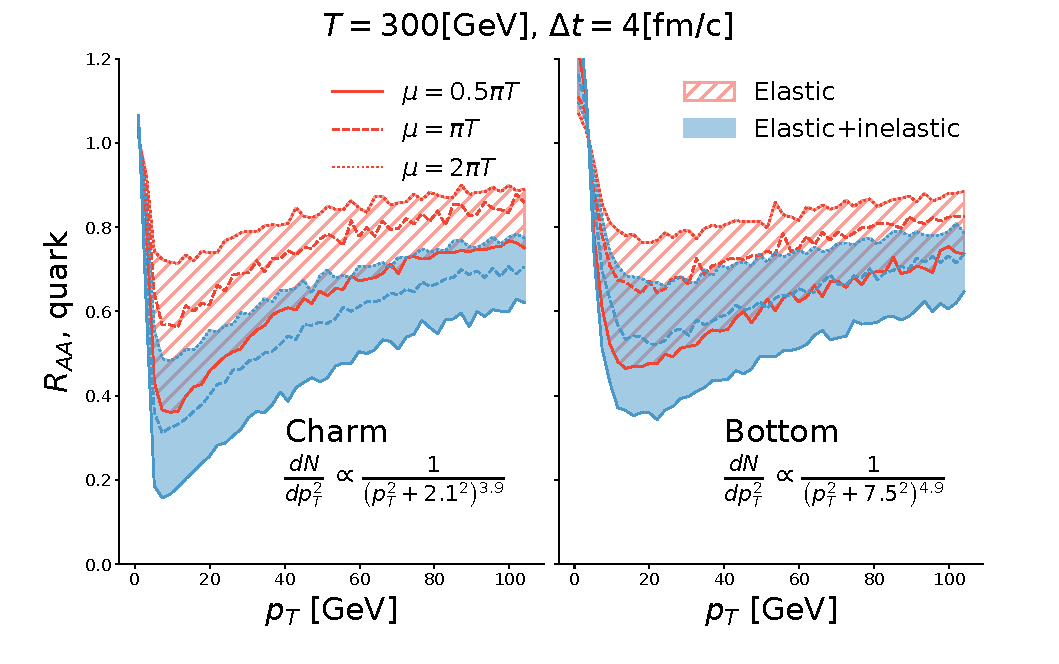
\includegraphics[width=\textwidth]{compare-plot/Box_Raa.pdf}
\end{figure*}

\section{Results}

\begin{appendices}
\section{Matrix elements}
\label{appendix:matrix-element}
\begin{widetext}
\begin{eqnarray}
\overline{|M_{Q+q\rightleftharpoons Q+q}|^2} &=& \frac{64\pi^2}{9}\alpha_s(t, T)^2 \frac{(u-M^2)^2 + (s-M^2)^2 + 2 M^2 t}{(t-m_D^2)^2}\\
\overline{|M_{Q+g\rightleftharpoons Q+g}|^2} &=& \pi^2 \left\{
32\alpha_s(t,T)^2 \frac{(s-M^2)(-u+M^2)}{(t-m_D^2)^2} \right. \\ \nonumber
&+&\frac{64}{9}\alpha_s(s-M^2, T)^2 \frac{(s-M^2)(-u+M^2)+2M*2(s-M^2) + 4M^4}{(s-M^2+m_D^2)^2} \\ \nonumber
&+&\frac{64}{9}\alpha_s(u-M^2, T)^2 \frac{(s-M^2)(-u+M^2)+2M*2(u-M^2) + 4M^4}{(-u+M^2+m_D^2)^2} \\ \nonumber
&+&\frac{16}{9}\alpha_s(u-M^2, T)\alpha_s(s-M^2, T) \frac{M^2(4M^2 - t)}{(-u+M^2+m_D^2)(s-M^2+m_D^2)} \\ \nonumber
&+& 16 \alpha_s(t, T)\alpha_s(s-M^2, T) \frac{(s-M^2)(-u+M^2)+M^2(s-u)}{(t-m_D^2)(s-M^2+m_D^2)} \\ \nonumber
&-& \left. 16 \alpha_s(t, T)\alpha_s(s-M^2, T) \frac{(s-M^2)(-u+M^2)-M^2(s-u)}{(t-m_D^2)(-u+M^2+m_D^2)}\right\} \\
\overline{|M_{Q+q\rightleftharpoons Q+q+g}|^2} &=& \overline{|M_{Q+g\rightleftharpoons Q+g}|^2} P_g \\
\overline{|M_{Q+g\rightleftharpoons Q+g+g}|^2} &=& \overline{|M_{Q+g\rightleftharpoons Q+g, \textrm{t-channel only}}|^2} P_g \\
P_g &=& 48 \pi \alpha_{s, \textrm{rad}} (1-\bar{x})^2 \left(\frac{\vec{k}_\perp}{k_\perp^2 + x^2 M^2 + (1-\bar{x})m_g^2} 
+ \frac{\vec{q}_\perp - \vec{k}_\perp}{(\vec{q}_\perp-\vec{k}_\perp)^2 + x^2 M^2 + (1-\bar{x})m_g^2}
\right)^2 
\end{eqnarray}
\end{widetext}

\section{Evolution with both scattering and diffusion dynamics}
With a transport $\hat{T} = -v\cdot \partial_x$, a scattering $\hat{C}$, and a diffusion $\hat{D}$ operator in the hybrid transport equation,
\begin{eqnarray}
\frac{\partial f}{\partial t} = \left( \hat{T} + \hat{C} + \hat{D} \right) f
\end{eqnarray}
The formal solution is,
\begin{eqnarray}
f_{\Delta t} = e^{\int_0^{\Delta t}  \left( \hat{T} + \hat{C} + \hat{D} \right) dt}f_0
\end{eqnarray}
Assume the time variance of the medium are slow and decompose the joint operation into separate operations.
\begin{eqnarray}
e^{ \Delta t\left(\hat{T} +\hat{C} + \hat{D} \right)} &=&
\nonumber
e^{\Delta t \left(\hat{T} + \hat{D}\right) } e^{\Delta t \hat{C}}   e^{-\frac{\Delta t^2}{2} [\hat{T}+\hat{D}, \hat{C}]}\left(1+O(\Delta t^3)\right) \\
\nonumber
&=& \frac{1}{2}  \left\{
1+\Delta t \left( \hat{T}+\hat{D} \right), 1+\Delta t C
\right\} + O(\Delta t^3) 
\end{eqnarray}
The operator $1 + \Delta t ( \hat{T}  + \hat{D} )$ stands for a ``Diffusion" step in the simulation; the operator $1+\Delta t \hat{C}$ stands for a ``Scattering" step in the simulation. 
Therefore, we design the following simulation procedure.
\begin{itemize}
\item For each step, choose a $\Delta t$ in lab frame small enough that total scattering probability $P_c \ll 1$.
\item Determine the ordering of diffusion step and scattering step with 50-50\% chance
\item If diffusion operates before scattering.
\begin{itemize}
\item[Step 1.] $(t, x, p) \xrightarrow{\textrm{Diffusion}} (t+\Delta t, x', p^*)$.
\item[Step 2.] $(t+\Delta t, x', p^*) \xrightarrow{\textrm{Scattering}} (t+\Delta t, x', p')$.
\end{itemize}
\item If diffusion operates after scattering.
\begin{itemize}
\item[Step 1.] $(t, x, p) \xrightarrow{\textrm{Scattering}} (t, x, p^*)$.
\item[Step 2.] $(t, x, p^*)  \xrightarrow{\textrm{Diffusion}} (t+\Delta t, x', p')$.
\end{itemize}
\end{itemize}

\section{Calculation of $\Raa$}
$\Raa$ is the ratio of differential cross-sections in AA collision to the that of pp collision scaled by the average number of binary collision for a given centrality.
The differential cross-sections has certain rapidity cuts.
Take the D-meson $\Raa$ as an example,
\begin{eqnarray}
\Raa = \frac{\left\langle \frac{dN_{AA \rightarrow D}}{dp_T}  \right\rangle_{|y|<y_0}}{\left. \langle T_{AA}\rangle \frac{d\sigma_{pp \rightarrow D}}{dp_T}\right|_{|y|<y_0}}
\end{eqnarray}
The average is taken over all events that fulfilling the centrality selection criterion.

This definition is straight forward in experiments because the differential cross-sections in the numerator and the denominator are measurable and $\langle T_{AA}\rangle$ is set of a model-dependent numbers.
For theory calculations there is more involved due to hadronization.
\begin{eqnarray}
\Raa &=& \frac{\left\langle \frac{T_{AA}}{\langle T_{AA}\rangle} \frac{d\sigma_{n n \rightarrow D}^{|y|<y_0}}{dp_T} \right\rangle}{ \frac{\sigma_{pp \rightarrow D}^{|y|<y_0}}{dp_T}} \\
&=& \frac{\left\langle \sigma_{nn \rightarrow D}^{|y|<y_0} \frac{d N_D^{|y|<y_0}}{dp_T} \right\rangle_{w=T_{AA}}}{\frac{d\sigma_{pp \rightarrow D}^{|y|<y_0}}{dp_T}}.
\end{eqnarray}
$d\sigma_{nn \rightarrow D}/dp_T$ is the D meson production within the rapidity cuts per binary collision.
$d N_D/dp_T$ is the normalized distribution of D meson in the final states which can be obtained directly from the transport simulation.
The average over events is then weighted by the nuclear overlapping function.
The missing piece that connects our calculation with the observable is the actually yield per binary collision of D meson for each event $\sigma_{nn\rightarrow D}$.
We relate this quantity to the initial charm production cross-section,
\begin{eqnarray}
\sigma_{nn\rightarrow D}^{|y|<y_0} &=& \sigma_{nn\rightarrow c}^{|y|<y_{max}} \frac{\sum_{|y|<y_0}w_D}{\sum_{|y|<y_{max}}w_c} \\
&=&  \sigma_{nn\rightarrow c}^{|y|<y_{max}} r_{D/c}.
\end{eqnarray}
$r_{D/c}$ can be calculate for each individual theory event, with $y_{max}>2y_0$ in actual calculations.
And the final theory calculation of $\Raa$ is,
\begin{eqnarray}
\Raa = \frac{\left\langle \sigma_{nn\rightarrow c}^{|y|<y_{max}} r_{D/c} \frac{d N_D^{|y|<y_0}}{dp_T} \right\rangle_{w=T_{AA}}}{\frac{d\sigma_{pp \rightarrow D}^{|y|<y_0}}{dp_T}}.
\end{eqnarray}

\section{Calculation of $v_n\{2\}$ and $v_2\{EP\}$}
Cumulant method correlates a heavy meson with a light particle to estimate $v_n$.
\begin{eqnarray}
v_n\{2\} &=& \frac{d_n\{2\}}{\sqrt{c_n\{2\}} } \\
d_n\{2\} &=& \left\langle \frac{\Re\{pQ^*\}}{mM} \right\rangle_{w = mM} \\
c_n\{2\} &=& \left\langle \frac{|Q|^2-M}{M(M-1)} \right\rangle_{w = M(M-1)}
\end{eqnarray}
\end{appendices}
\end{document}